\begin{figure}[h!]
\tikzset{every picture/.style={line width=0.75pt}} %set default line width to 0.75pt        

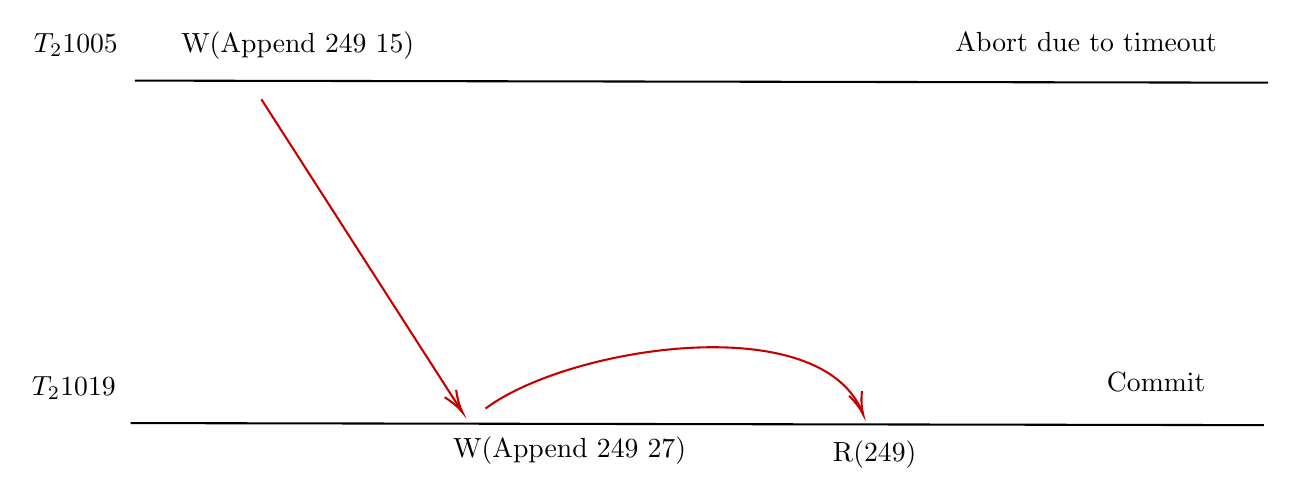
\begin{tikzpicture}[x=0.75pt,y=0.75pt,yscale=-1,xscale=1]
%uncomment if require: \path (0,300); %set diagram left start at 0, and has height of 300

%Straight Lines [id:da9500410641573396] 
\draw    (62.09,31) -- (608.09,32) ;
%Straight Lines [id:da7796185686481738] 
\draw    (60.09,196) -- (606.09,197) ;
%Straight Lines [id:da424831019884359] 
\draw [color={rgb, 255:red, 198; green, 0; blue, 0 }  ,draw opacity=1 ]   (123.09,40) -- (219,189.32) ;
\draw [shift={(220.09,191)}, rotate = 237.28] [color={rgb, 255:red, 198; green, 0; blue, 0 }  ,draw opacity=1 ][line width=0.75]    (10.93,-3.29) .. controls (6.95,-1.4) and (3.31,-0.3) .. (0,0) .. controls (3.31,0.3) and (6.95,1.4) .. (10.93,3.29)   ;
%Curve Lines [id:da475730388715653] 
\draw [color={rgb, 255:red, 198; green, 0; blue, 0 }  ,draw opacity=1 ]   (231.09,189) .. controls (270.69,159.3) and (391.63,140.38) .. (412.48,190.46) ;
\draw [shift={(413.09,192)}, rotate = 249.93] [color={rgb, 255:red, 198; green, 0; blue, 0 }  ,draw opacity=1 ][line width=0.75]    (10.93,-3.29) .. controls (6.95,-1.4) and (3.31,-0.3) .. (0,0) .. controls (3.31,0.3) and (6.95,1.4) .. (10.93,3.29)   ;

% Text Node
\draw (12,7) node [anchor=north west][inner sep=0.75pt]   [align=left] {$T_21005$};
% Text Node
\draw (11,172) node [anchor=north west][inner sep=0.75pt]   [align=left] {$T_21019$};
% Text Node
\draw (83,6) node [anchor=north west][inner sep=0.75pt]   [align=left] {W(Append 249 15)};
% Text Node
\draw (214,201) node [anchor=north west][inner sep=0.75pt]   [align=left] {W(Append 249 27)};
% Text Node
\draw (397,203) node [anchor=north west][inner sep=0.75pt]   [align=left] {R(249)};
% Text Node
\draw (456,6) node [anchor=north west][inner sep=0.75pt]   [align=left] {Abort due to timeout};
% Text Node
\draw (529,170) node [anchor=north west][inner sep=0.75pt]   [align=left] {Commit};
% Text Node
\draw (120,130) node [anchor=north west][inner sep=0.75pt]   [align=left] {};

\end{tikzpicture}
\caption{G0: Dirt write violation that occurred during one of the runs.}
\end{figure}
